
%(BEGIN_QUESTION)
% Copyright 2009, Tony R. Kuphaldt, released under the Creative Commons Attribution License (v 1.0)
% This means you may do almost anything with this work of mine, so long as you give me proper credit

Use loop simulation software on a personal computer to simulate the effects of an ``open loop'' test.  This means placing the loop controller in manual mode and moving the control valve by 5\% or 10\%.  Try this on a simulated process of your own choosing (browse the software's available process types) and sketch the results.  {\it Answer this question for a process you have not done an open loop test on yet:}

$$\includegraphics[width=15.5cm]{i04321x01.eps}$$

Determine whether the process is self-regulating or integrating.  If it is self-regulating, determine its steady-state gain by dividing the change in PV by the change in output ($\Delta \hbox{PV} \over \Delta m$):

\vskip 10pt

Steady-state gain = \underbar{\hskip 50pt} with valve step-change from \underbar{\hskip 50pt}\% to \underbar{\hskip 50pt}\%

\vskip 10pt

Steady-state gain = \underbar{\hskip 50pt} with valve step-change from \underbar{\hskip 50pt}\% to \underbar{\hskip 50pt}\%

\vskip 10pt

Steady-state gain = \underbar{\hskip 50pt} with valve step-change from \underbar{\hskip 50pt}\% to \underbar{\hskip 50pt}\%


\vskip 20pt \vbox{\hrule \hbox{\strut \vrule{} {\bf Suggestions for Socratic discussion} \vrule} \hrule}

\begin{itemize}
\item{} Why should an {\it open-loop} test be one of the first things you do when attempting to optimize a control loop?
\end{itemize}

\underbar{file i04321}
%(END_QUESTION)





%(BEGIN_ANSWER)


%(END_ANSWER)





%(BEGIN_NOTES)

%INDEX% Control, process characteristics: computer simulation software (process gains)

%(END_NOTES)

